\chapter{Path Planning}

\paragraph*{}
Path planning algorithm used for our swarm is exactly the same one as the one used in the simulation in the previous semester. However, we have also implemented a converter of the original paths, which is a collection of coordinates the robots should move towards in each timestep, to a collection of directions and how much time the robots should move to that particular direction (Figure \ref{fig:path-without-obstacles}). This has been done to make communication between the swarm more efficient by effectively reducing the message size, allowing for both speed and eliminating the need for an excessively large buffer size for the receiving end of the communication.

\begin{figure} [H]
    \centering
    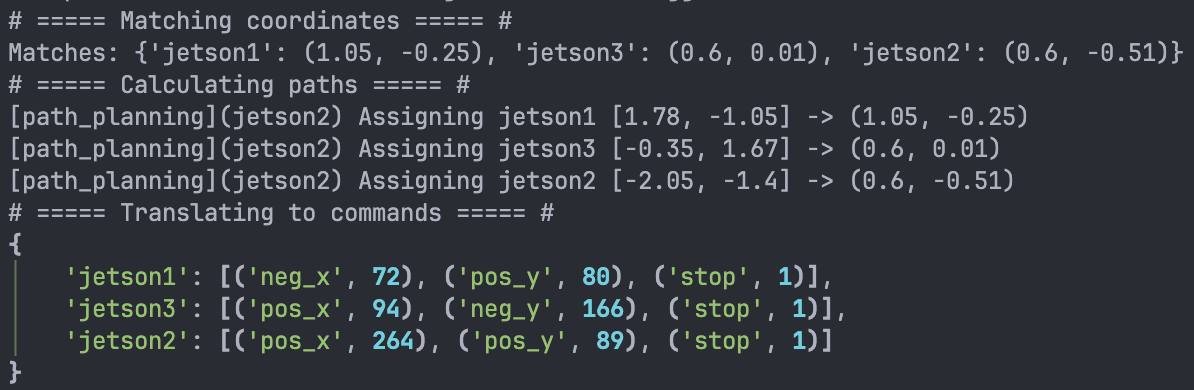
\includegraphics[width=0.9\linewidth]{assets/images/path_planning/path_without_obstacles.png}
    \caption{Output of the Path Planning Algorithm}
    \label{fig:path-without-obstacles}
\end{figure}

\paragraph*{}
The path planning algorithm for the swarm is designed to be collisionless, with a functional obstacle avoidance plan. We ensure collisionless paths by implementing the plan so that if in a single timestep, the coordinates the robot is planning to move has already been taken by another, it will stay stationary for that particular timestep to avoid collisions within the swarm. While ensuring collisionless paths, obstacles can also be avoided by planning the paths to go around any obstacles in the path. Figure \ref{fig:path-without-obstacles} shows planning for three swarm members to surround a detected object without any obstacles, whereas Figure \ref{fig:path-with-obstacles} illustrates the same planning with respect to the starts and the destinations, but with manually added obstacles along the intended path. The flow for the path planning is attached below. (Figure \ref{fig:path-planning-flow})

\begin{figure} [H]
    \centering
    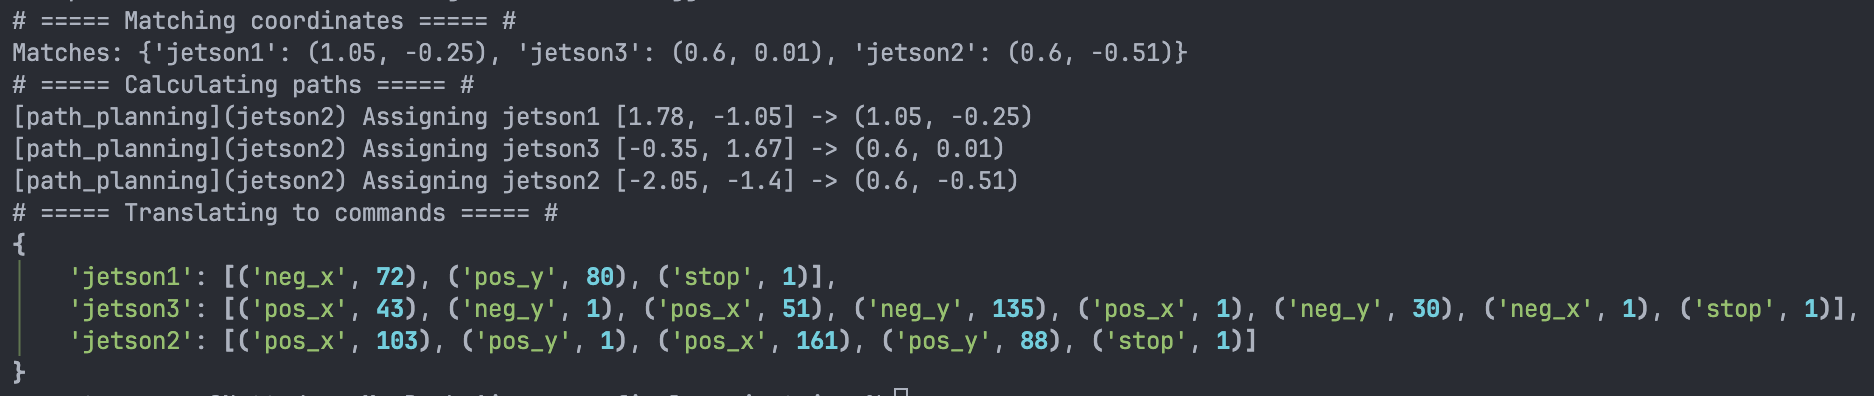
\includegraphics[width=0.9\linewidth]{assets/images/path_planning/path_with_obstacles.png}
    \caption{Path Planning with Obstacles}
    \label{fig:path-with-obstacles}
\end{figure}

\begin{figure} [H]
    \centering
    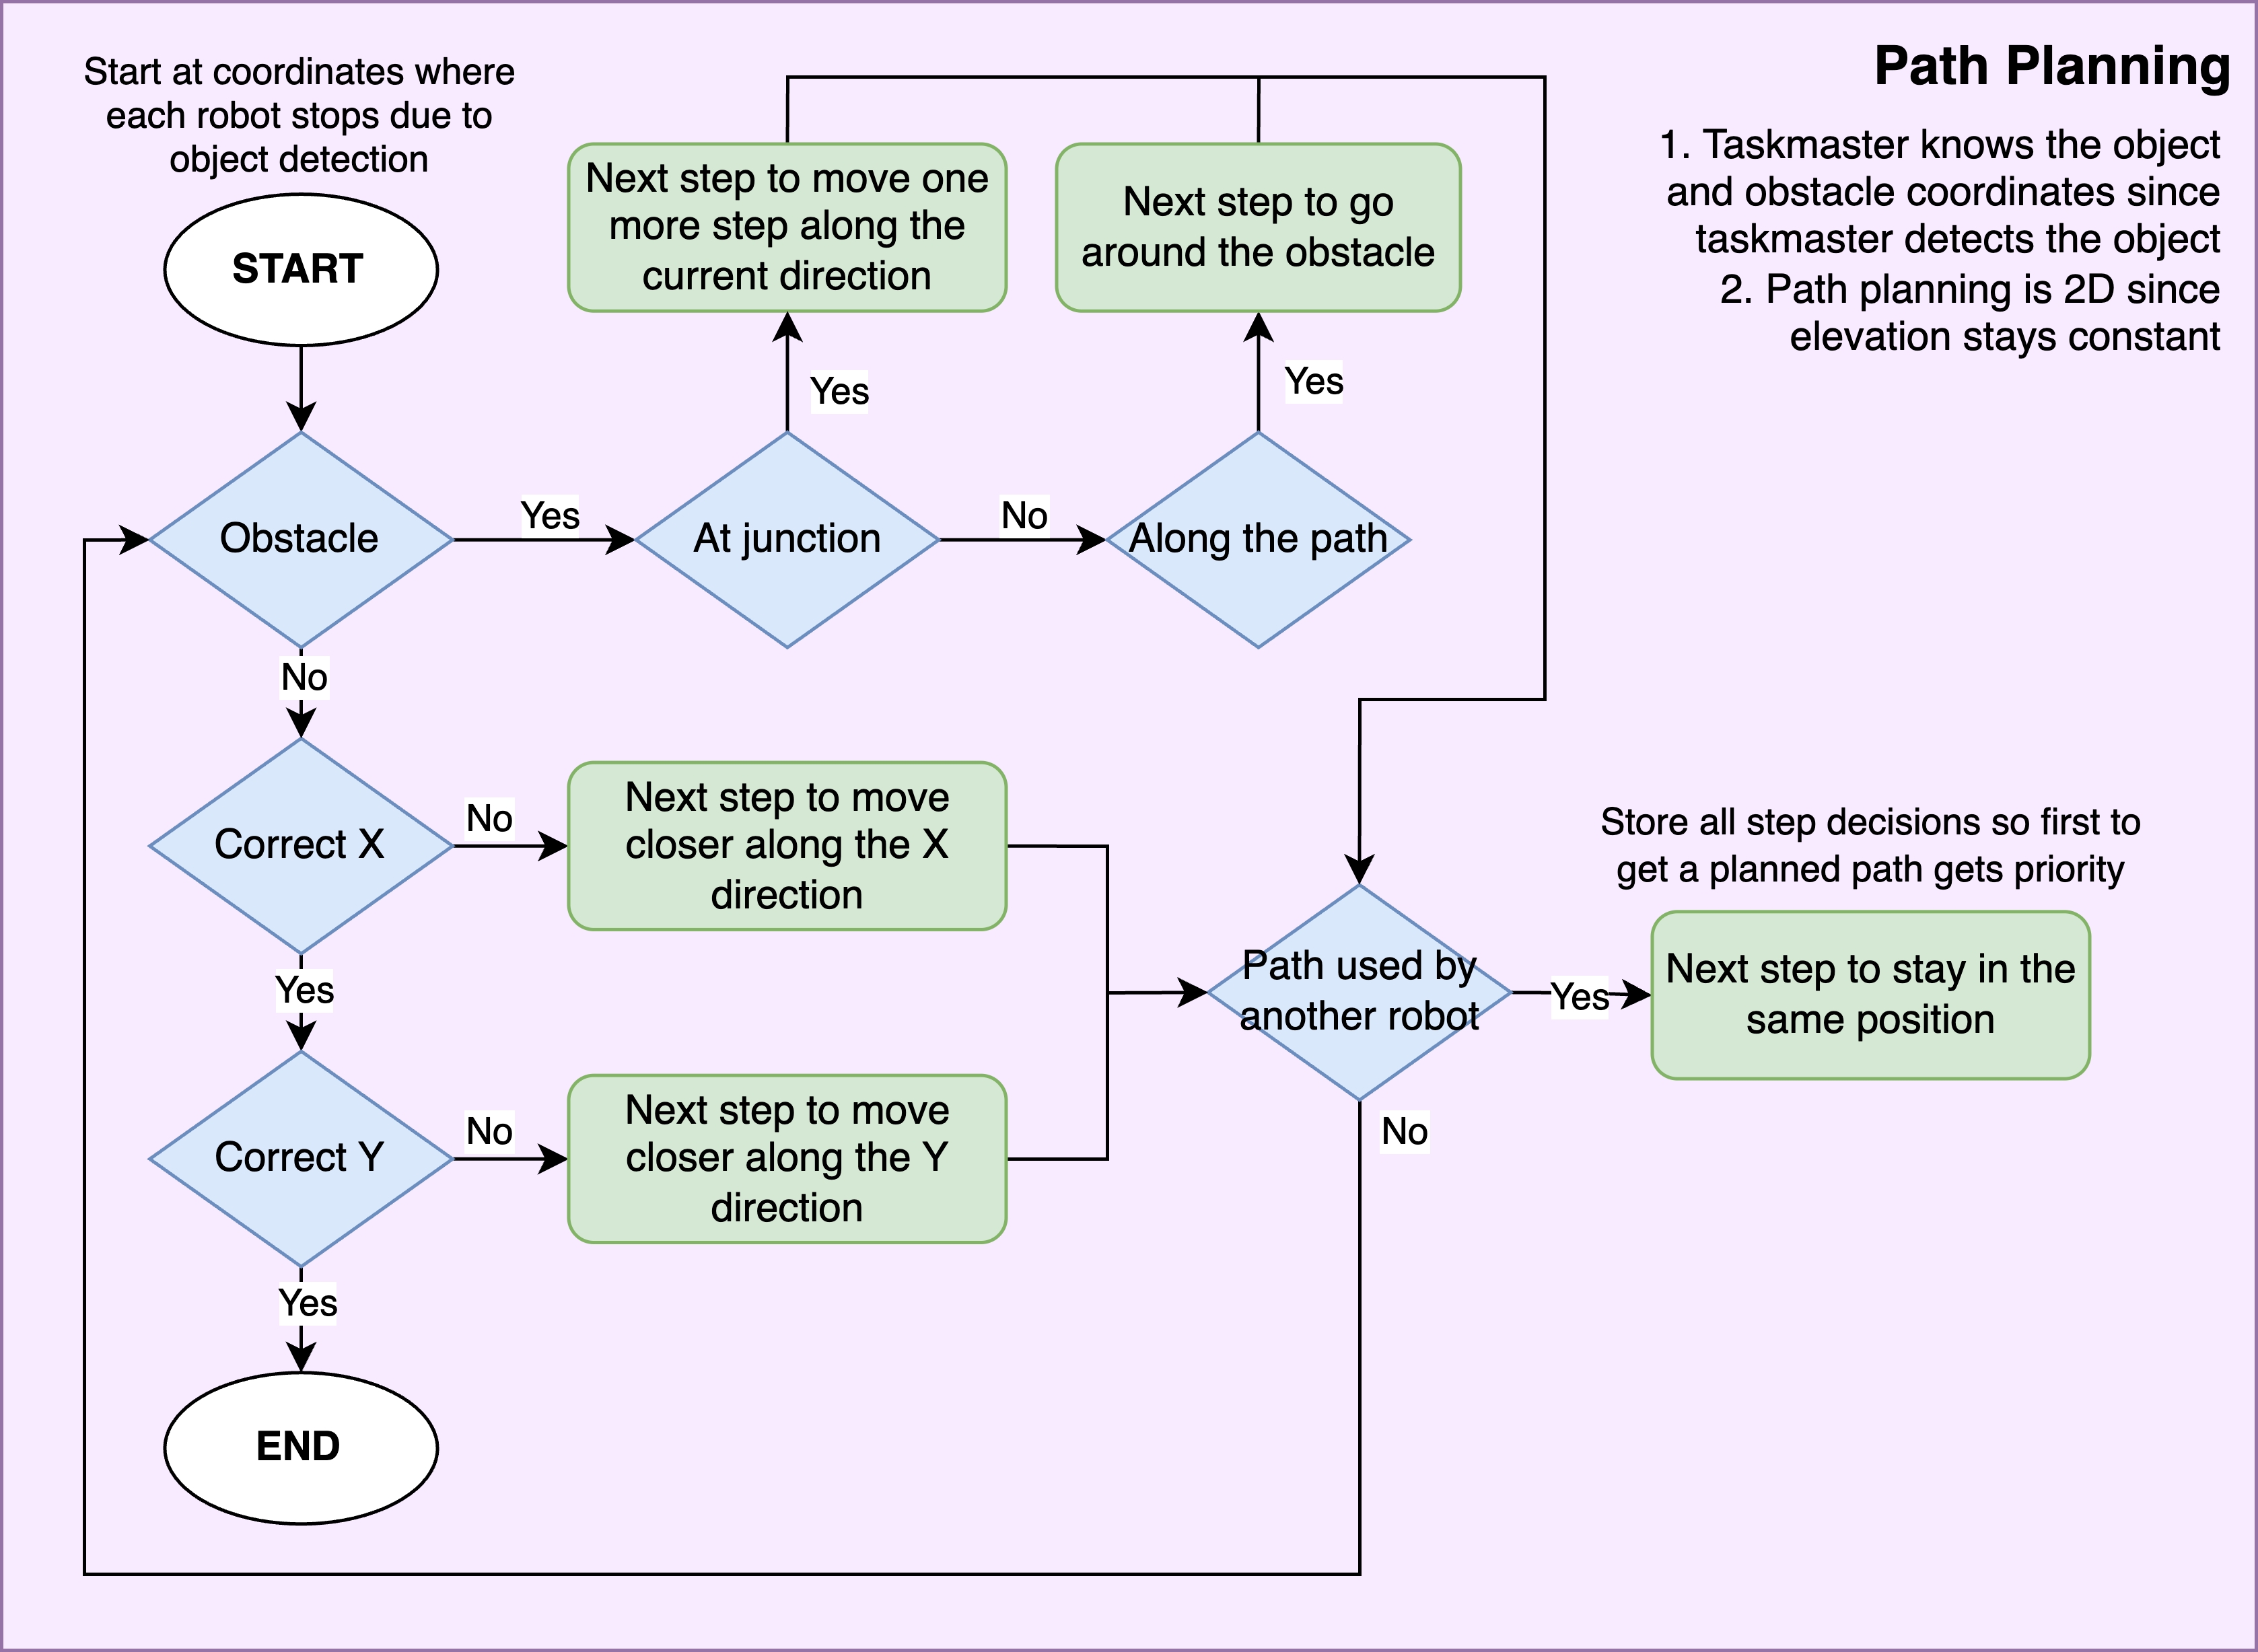
\includegraphics[width=0.9\linewidth]{assets/images/path_planning/path-planning-flow.png}
    \caption{Path Planning Detailed Flow}
    \label{fig:path-planning-flow}
\end{figure}
